\documentclass{beamer}

%Packages BEGIN
\usepackage{amsmath}
\usepackage{xeCJK} % use this package to set Chinese and English font separately
\usepackage{fontspec} 
 

%Packages END

%Style setting BEGIN
\usetheme{Madrid} 
\usecolortheme{default} 

% Serif font in Ubuntu. Choose the Chinese font available in your device
\setCJKmainfont{Noto Serif CJK TC}

% Serif font in Ubuntu. Choose the Chinese font available in your device
\setCJKmonofont{Noto Serif CJK TC}

% Serif font in Ubuntu. Choose the Chinese font available in your device
\setCJKsansfont{Noto Serif CJK TC}

\XeTeXlinebreaklocale "zh" % enabling auto linebreaks
\XeTeXlinebreakskip = 0pt plus 1pt % enabling auto linebreaks
 
%Style setting END


\begin{document}

\frame{\titlepage} 

\begin{frame}
	\frametitle{Image Recognization}
	\textbf{Goal}: Indentify the word in the picture and use it to generate the card.
	\begin{figure}[h]`
		\centering
		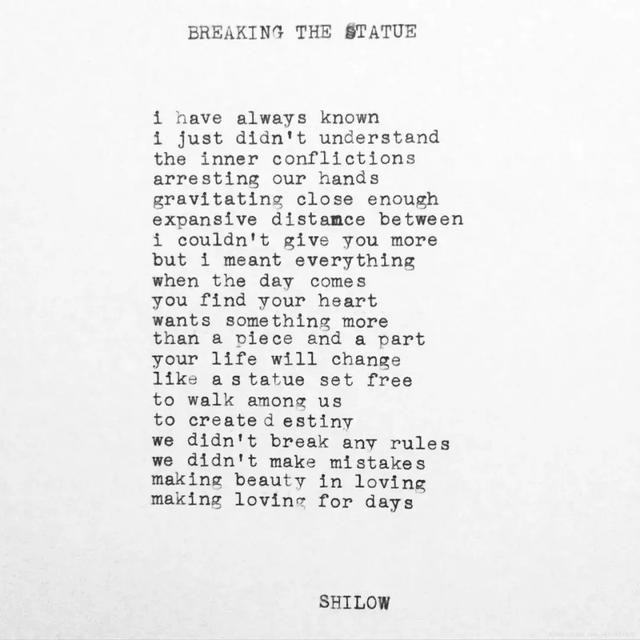
\includegraphics[width=0.55\linewidth]{./img1.jpg}
		\caption{Target picture}
	\end{figure}
\end{frame}

\begin{frame}{Method}
		\textbf{Step1}: Convert the picture to gray color. Then, set the blacker one to total black, whiter one to total white.\\
		\textbf{Step1-1}: To realize step1, we would turn the picture into array to deal with it.
		\begin{figure}[h]
			\centering
			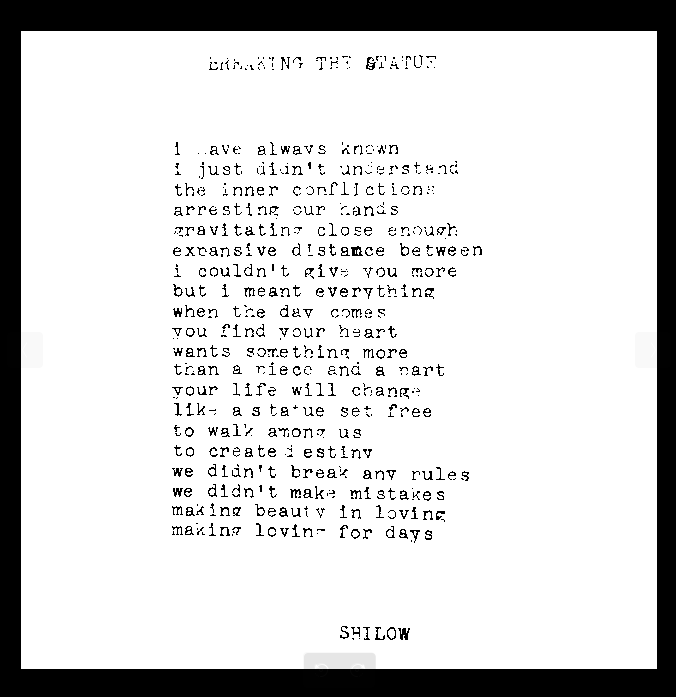
\includegraphics[width=0.50\linewidth]{./picture_blackwhite.png}
		\end{figure}
\end{frame}

\begin{frame}{Task}
		\textbf{How computer see a word?}
		\begin{figure}[h]
			\centering
			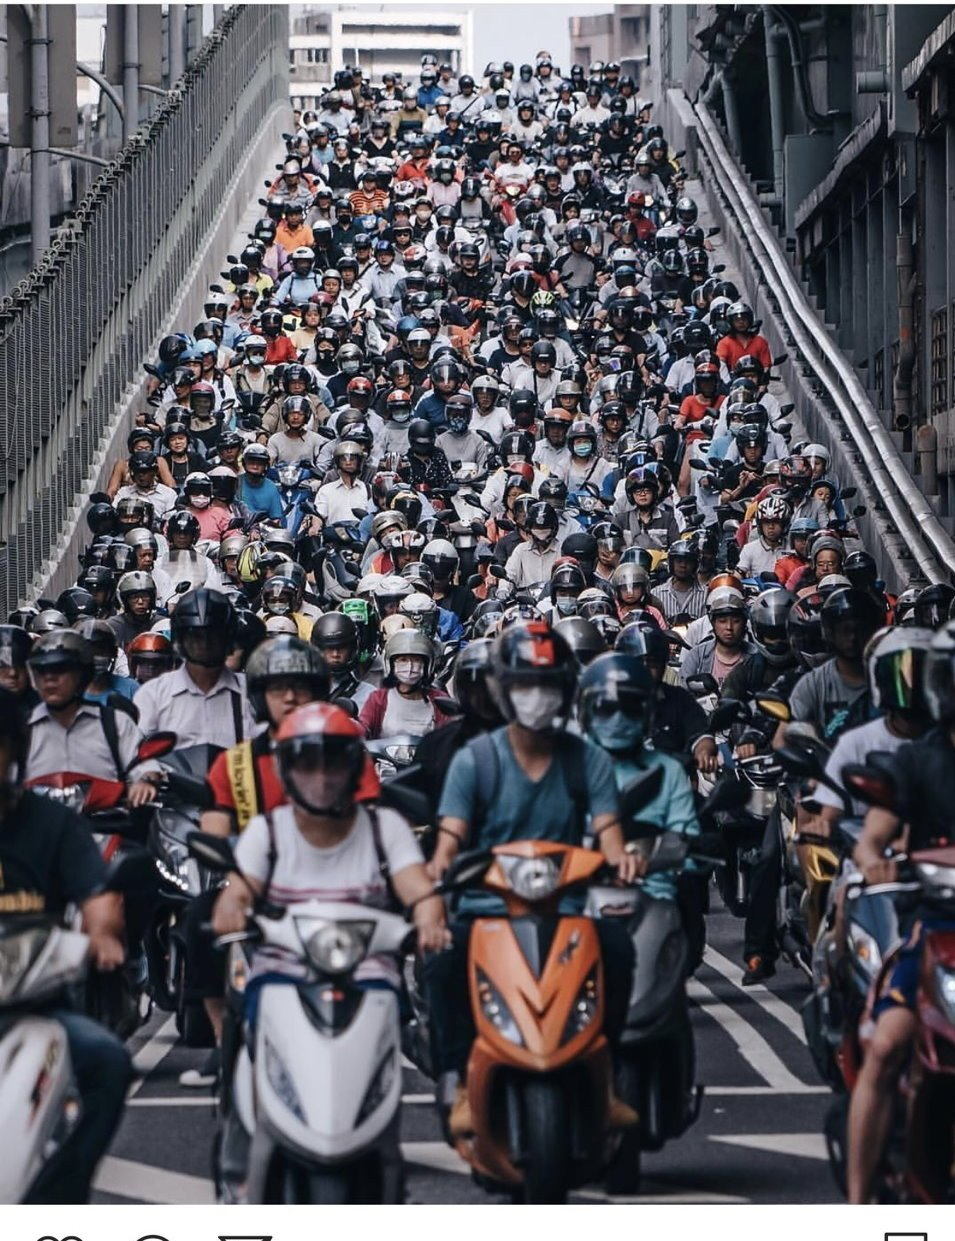
\includegraphics[width=0.55\linewidth]{./motor.jpg}
		\end{figure}
\end{frame}

\begin{frame}{Fourier Transform}
		\textbf{It seems good but awful.}
		\begin{figure}[H]
			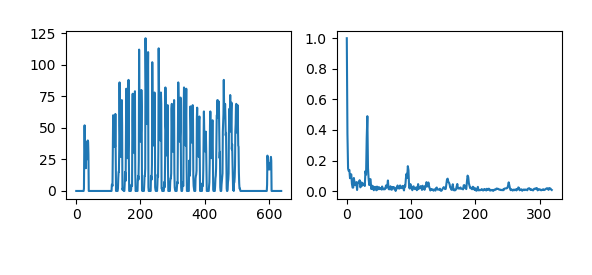
\includegraphics[width=0.45\linewidth]{./fourier.png}
			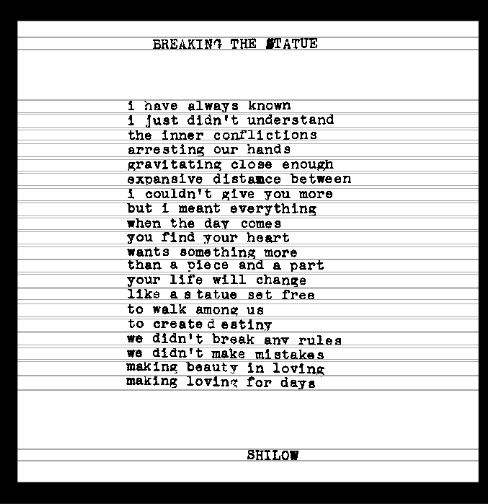
\includegraphics[width=0.55\linewidth]{./imgslice.png}
		\end{figure}
\end{frame}

\begin{frame}{Fourier Transform}
	\textbf{Fewer data lead to less precision.}
	\begin{figure}[H]
		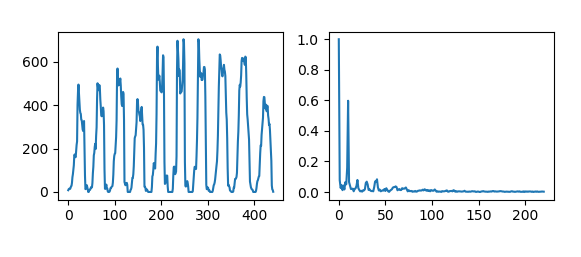
\includegraphics[width=0.55\linewidth]{./fourier2.png}
		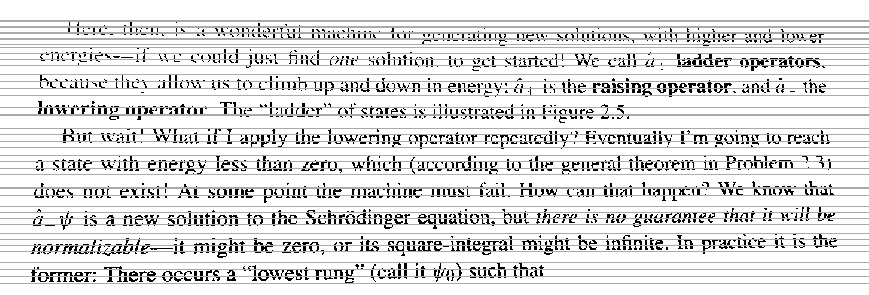
\includegraphics[width=0.70\linewidth]{./imgslice2.png}
	\end{figure}
\end{frame}

\begin{frame}{Method}
		\textbf{Step2-1}: When the black pixels number is below the threshold number, recognize it as a white raw. This can help us detect the line.\\
		\textbf{Step2-2}: Analyze the line, detect the wider white column to recognize the word.\\
		\begin{figure}[h]
			\centering
			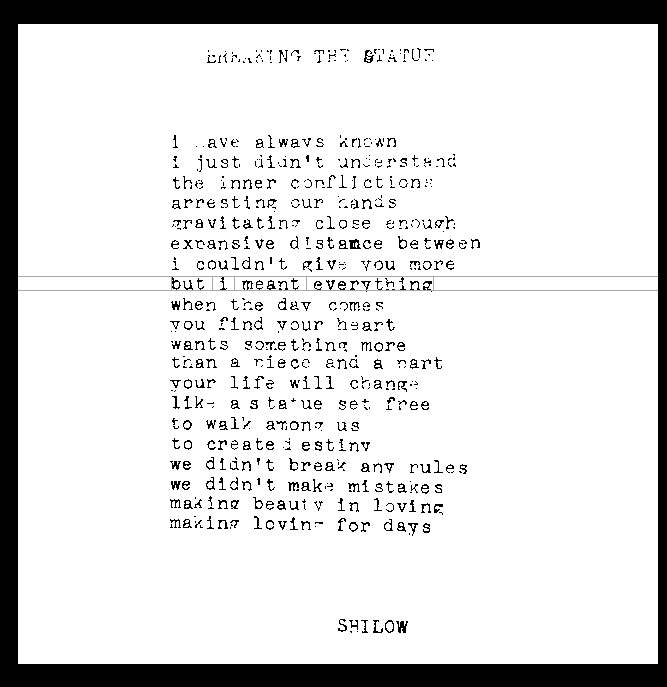
\includegraphics[width=0.50\linewidth]{./raw_done.png}
		\end{figure}
\end{frame}

\begin{frame}{Method}
		\textbf{Step3-1}: Detect the words in the line, use the order to determine which word I selected. We get WordFromLine.\\
		\textbf{Step3-2}: Detect the word in the region I selected. We get WordFromWord.\\
		\textbf{Step3-3}: If the WordFromLine is similar to WordFromWord or len(WordFromWord)=0, return WordFromLine. Else, return WordFromWord.\\
		\begin{figure}[h]
			\centering
			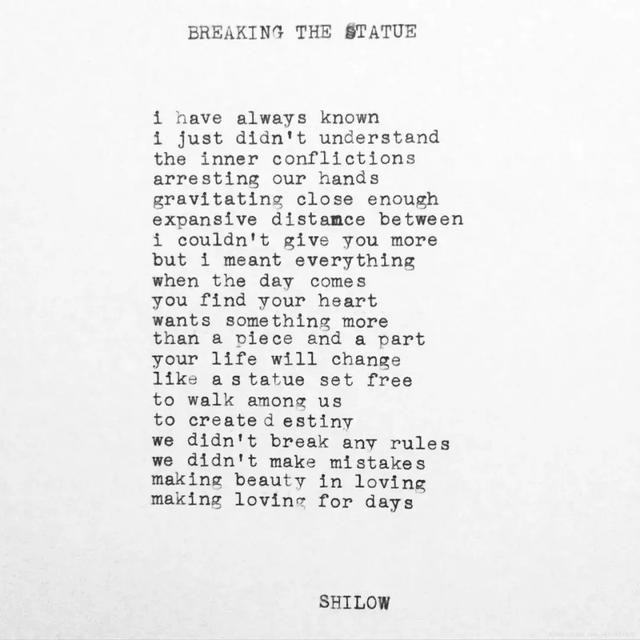
\includegraphics[height=0.4\linewidth]{./img1.jpg}
			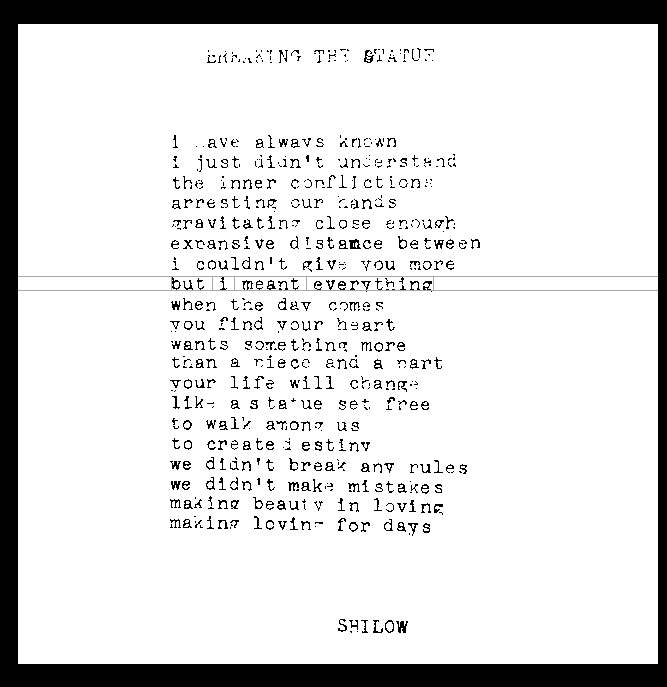
\includegraphics[width = 0.4\linewidth]{./raw_done.png}
		\end{figure}
\end{frame}

\end{document}
